\documentclass[aps,prl,floatfix,twocolumn,footinbib,superscriptaddress]{revtex4-1}
%DIF LATEXDIFF DIFFERENCE FILE
%DIF DEL QDNVold.tex   Fri May 10 16:55:02 2019
%DIF ADD QDNV.tex      Wed Aug  7 15:13:12 2019
\usepackage{epsfig}
\usepackage{float}
\usepackage{epstopdf} %converting to PDF
\usepackage{braket}
\usepackage[utf8]{inputenc}
\usepackage{amsmath}
\usepackage{amssymb}
\usepackage{esint}
\usepackage{xcolor}
\usepackage{bbm}
%DIF PREAMBLE EXTENSION ADDED BY LATEXDIFF
%DIF UNDERLINE PREAMBLE %DIF PREAMBLE
\RequirePackage[normalem]{ulem} %DIF PREAMBLE
\RequirePackage{color}\definecolor{RED}{rgb}{1,0,0}\definecolor{BLUE}{rgb}{0,0,1} %DIF PREAMBLE
\providecommand{\DIFadd}[1]{{\protect\color{blue}\uwave{#1}}} %DIF PREAMBLE
\providecommand{\DIFdel}[1]{{\protect\color{red}\sout{#1}}}                      %DIF PREAMBLE
%DIF SAFE PREAMBLE %DIF PREAMBLE
\providecommand{\DIFaddbegin}{} %DIF PREAMBLE
\providecommand{\DIFaddend}{} %DIF PREAMBLE
\providecommand{\DIFdelbegin}{} %DIF PREAMBLE
\providecommand{\DIFdelend}{} %DIF PREAMBLE
\providecommand{\DIFmodbegin}{} %DIF PREAMBLE
\providecommand{\DIFmodend}{} %DIF PREAMBLE
%DIF FLOATSAFE PREAMBLE %DIF PREAMBLE
\providecommand{\DIFaddFL}[1]{\DIFadd{#1}} %DIF PREAMBLE
\providecommand{\DIFdelFL}[1]{\DIFdel{#1}} %DIF PREAMBLE
\providecommand{\DIFaddbeginFL}{} %DIF PREAMBLE
\providecommand{\DIFaddendFL}{} %DIF PREAMBLE
\providecommand{\DIFdelbeginFL}{} %DIF PREAMBLE
\providecommand{\DIFdelendFL}{} %DIF PREAMBLE
%DIF LISTINGS PREAMBLE %DIF PREAMBLE
\RequirePackage{listings} %DIF PREAMBLE
\RequirePackage{color} %DIF PREAMBLE
\lstdefinelanguage{DIFcode}{ %DIF PREAMBLE
%DIF DIFCODE_UNDERLINE %DIF PREAMBLE
  moredelim=[il][\color{red}\sout]{\%DIF\ <\ }, %DIF PREAMBLE
  moredelim=[il][\color{blue}\uwave]{\%DIF\ >\ } %DIF PREAMBLE
} %DIF PREAMBLE
\lstdefinestyle{DIFverbatimstyle}{ %DIF PREAMBLE
	language=DIFcode, %DIF PREAMBLE
	basicstyle=\ttfamily, %DIF PREAMBLE
	columns=fullflexible, %DIF PREAMBLE
	keepspaces=true %DIF PREAMBLE
} %DIF PREAMBLE
\lstnewenvironment{DIFverbatim}{\lstset{style=DIFverbatimstyle}}{} %DIF PREAMBLE
\lstnewenvironment{DIFverbatim*}{\lstset{style=DIFverbatimstyle,showspaces=true}}{} %DIF PREAMBLE
%DIF END PREAMBLE EXTENSION ADDED BY LATEXDIFF

\begin{document}

\global\long\def\avg#1{\langle#1\rangle}

\global\long\def\p{\prime}

\global\long\def\dg{\dagger}

\global\long\def\ket#1{|#1\rangle}

\global\long\def\bra#1{\langle#1|}

\global\long\def\proj#1#2{|#1\rangle\langle#2|}

\global\long\def\inner#1#2{\langle#1|#2\rangle}

\global\long\def\tr{\mathrm{tr}}

\global\long\def\pd#1#2{\frac{\partial#1}{\partial#2}}

\global\long\def\spd#1#2{\frac{\partial^{2}#1}{\partial#2^{2}}}

\global\long\def\der#1#2{\frac{d#1}{d#2}}

\global\long\def\im{\imath}

\global\long\def\S{\mathcal{S}}

\global\long\def\A{\mathcal{A}}

\global\long\def\F{\mathcal{F}}

\global\long\def\E{\mathcal{E}}

\global\long\def\As{{^{\sharp}}\hspace{-1mm}\mathcal{A}}

\global\long\def\Fs{{^{\sharp}}\hspace{-0.7mm}\mathcal{F}}

\global\long\def\Es{{^{\sharp}}\hspace{-0.5mm}\mathcal{E}}

\global\long\def\EsG{{^{\sharp}}\hspace{-0.5mm}\mathcal{E}_{G}}

\global\long\def\EsB{{^{\sharp}}\hspace{-0.5mm}\mathcal{E}_{B}}

\global\long\def\FsG{{^{\sharp}}\hspace{-0.5mm}\F_{G}}

\global\long\def\FsB{{^{\sharp}}\hspace{-0.5mm}\F_{B}}

\global\long\def\Fd{{^{\sharp}}\hspace{-0.7mm}\mathcal{F}_{\delta}}

\global\long\def\EG{\mathcal{E}_{G}}

\global\long\def\EB{\mathcal{E}_{B}}

\global\long\def\O{\mathcal{O}}

\global\long\def\SgF{\S d\F}

\global\long\def\SgEF{\S d\left(\E/\F\right)}

\global\long\def\U{\mathcal{U}}

\global\long\def\V{\mathcal{V}}

\global\long\def\H{\mathbf{H}}

\global\long\def\SO{\Pi_{\S}}

\global\long\def\PO{\hat{\Pi}_{\S}}

\global\long\def\SSH{\tilde{\Pi}_{\S}}

\global\long\def\EO{\Upsilon_{k}}

\global\long\def\ESH{\Omega_{k}}

\global\long\def\HSF{\mathbf{H}_{\S\F}}

\global\long\def\HSEF{\mathbf{H}_{\S\E/\F}}

\global\long\def\HS{\mathbf{H}_{\S}}

\global\long\def\ES{H_{\S}(t)}

\global\long\def\ESo{H_{\S}(0)}

\global\long\def\EgF{H_{\SgF} (t)}

\global\long\def\EgE{H_{\S d\E}(t)}

\global\long\def\EgEF{H_{\SgEF} (t)}

\global\long\def\EF{H_{\F}(t)}

\global\long\def\EFo{H_{\F}(0)}

\global\long\def\ESF{H_{\S\F}(t)}

\global\long\def\ESEF{H_{\S\E/\F}(t)}

\global\long\def\ESSEF{H_{\tilde{\S}\S\E/\F}(t)}

\global\long\def\EEFo{H_{\E/\F}(0)}

\global\long\def\EEF{H_{\E/\F}(t)}

\global\long\def\HPB{H(\PB)}

\global\long\def\MI{I\left(\S:\F\right)}

\global\long\def\aMI{\left\langle \MI\right\rangle _{\Fs}}

\global\long\def\BS{\Pi_{\S} }

\global\long\def\PB{\hat{\Pi}_{\S} }

\global\long\def\QD{\mathcal{D}\left(\Pi_{\S}:\F\right)}
\global\long\def\QD{\mathcal{D}(\Pi_{\S}:\F)}

\global\long\def\QDp{\mathcal{D}\left(\PB:\F\right)}
\global\long\def\QDpIL{\mathcal{D}(\PB:\F)}

\global\long\def\JI{J\left(\Pi_{\S}:\F\right)}

\global\long\def\CI{H\left(\F\left|\Pi_{\S}\right.\right)}

\global\long\def\CIp{H\left(\F\left|\PB\right.\right)}

\global\long\def\CS{\rho_{\F\left|s\right.}}

\global\long\def\CSu{\tilde{\rho}_{\F\left|s\right.}}

\global\long\def\CSp{\rho_{\F\left|\hat{s}\right.}}

\global\long\def\CEF{H_{\F\left|s\right.}}

\global\long\def\CEFp{H_{\F\left|\hat{s}\right.}}

\global\long\def\psiz{\ket{\psi_{\E\left|0\right.\hspace{-0.4mm}}}}

\global\long\def\psio{\ket{\psi_{\E\left|1\right.\hspace{-0.4mm}}}}

\global\long\def\psiinner{\inner{\psi_{\E\left|0\right.\hspace{-0.4mm}}}{\psi_{\E\left|1\right.\hspace{-0.4mm}}}}

\global\long\def\QDz{\boldsymbol{\delta}\left(\S:\F\right)_{\left\{  \sigma_{\S}^{z}\right\}  }}

\global\long\def\NQD{\bar{\boldsymbol{\delta}}\left(\S:\F\right)_{\BS}}

\global\long\def\EFS{H_{\F\left| \BS\right. }(t)}

\global\long\def\EFSM{H_{\F\left| \left\{  \ket m\right\}  \right. }(t)}

\global\long\def\Hol{\chi\left(\Pi_{\S}:\F\right)}
\global\long\def\HolIL{\chi (\Pi_{\S}:\F) }

\global\long\def\Holp{\chi\left(\PB:\F\right)}
\global\long\def\HolpIL{\chi ( \PB:\F )}

\global\long\def\ch{\raisebox{0.5ex}{\mbox{\ensuremath{\chi}}}_{\mathrm{Pointer}}}

\global\long\def\rhoS{\rho_{\S}(t)}

\global\long\def\rhoSo{\rho_{\S}(0)}

\global\long\def\rhoSF{\rho_{\S\F} (t)}

\global\long\def\rhoSgEF{\rho_{\SgEF} (t)}

\global\long\def\rhoSgF{\rho_{\SgF} (t)}

\global\long\def\rhoF{\rho_{\F}(t)}

\global\long\def\rhoFp{\rho_{\F}(\pi/2)}

\global\long\def\LE{\Lambda_{\E}(t)}

\global\long\def\LEc{\Lambda_{\E}^{\star}(t)}

\global\long\def\LEij{\Lambda_{\E}^{ij}(t)}

\global\long\def\LF{\Lambda_{\F}(t)}

\global\long\def\LFij{\Lambda_{\F}^{ij} (t)}

\global\long\def\LFc{\Lambda_{\F}^{\star}(t)}

\global\long\def\LEF{\Lambda_{\E/\F} (t)}

\global\long\def\LEFij{\Lambda_{\E/\F}^{ij}(t)}

\global\long\def\LEFc{\Lambda_{\E/\F}^{\star}(t)}

\global\long\def\Lkij{\Lambda_{k}^{ij}(t)}

\global\long\def\Hb{H}

\global\long\def\kE{\kappa_{\E}(t)}

\global\long\def\kEF{\kappa_{\E/\F}(t)}

\global\long\def\kF{\kappa_{\F}(t)}

\global\long\def\ts{t=\pi/2}

\global\long\def\QCB{\bar{\xi}_{QCB}}

\global\long\def\mc#1{\mathcal{#1}}

\global\long\def\MD{\lambda}

\global\long\def\up{\mathord{\uparrow}}

\global\long\def\down{\mathord{\downarrow}}

\global\long\def\Cku{\rho_{k\left|\up\right.}}

\global\long\def\Ckd{\rho_{k\left|\down\right.}}

\global\long\def\f{\mathcal{J}}

\global\long\def\onlinecite#1{\cite{#1}}

\newcommand{\todo}[1]{\textcolor{red}{#1}}
\newcommand{\RN}[1]{\uppercase\expandafter{\romannumeral#1}}

\title{Revealing the emergence of classicality in nitrogen-vacancy centers}

%Alt titles: 
%\title{Revealing the emergence of the classicality via NV center measurements}
%Revealing the emergence of the classical world via NV center measurements
%The emergence of a classical NV-center spin /via nuclear-spin decoherence
%The emergence of redundancy in nuclear spin environments of an NV center.
%Quantum Darwinism in action (in the lab): The emergence of redundancy in nuclear spin environments of an NV center.

\author{T. K. Unden}
\affiliation{Institute for Quantum Optics, Ulm University, Albert-Einstein-Allee 11, Ulm 89081, Germany}
\DIFdelbegin %DIFDELCMD < \affiliation{Hensoldt Sensor Solutions GmbH, Woerthstrasse 85, Ulm 89077, Germany}
%DIFDELCMD < %%%
\DIFdelend \author{D. Louzon}
\affiliation{Institute for Quantum Optics, Ulm University, Albert-Einstein-Allee 11, Ulm 89081, Germany}
\affiliation{Racah Institute of Physics, The Hebrew University of Jerusalem, Jerusalem 91904, Israel}

\author{M. Zwolak}
\affiliation{Biophysics Group, Microsystems and Nanotechnology Division, Physical Measurement Laboratory, National Institute of Standards and Technology, Gaithersburg,
Maryland 20899, U.S.A.}

\author{W. H. Zurek}
\affiliation{Theory Division, Los Alamos National Laboratory, Los Alamos, NM, 87545, U.S.A.}

\author{F. Jelezko}
\affiliation{Institute for Quantum Optics, Ulm University, Albert-Einstein-Allee 11, Ulm 89081, Germany}
\affiliation{Center for Integrated Quantum Science and Technology (IQ$^\text{{st}}$), Ulm University, 89081 Germany}



\begin{abstract}
{
The origin of classical reality in our quantum world is a long-standing mystery. Here, we examine a nitrogen vacancy center \DIFdelbegin \DIFdel{evolving }%DIFDELCMD < {\em %%%
\DIFdel{naturally}%DIFDELCMD < } %%%
\DIFdelend \DIFaddbegin \DIFadd{in diamond evolving }\DIFaddend in the presence of its \DIFdelbegin \DIFdel{environment }\DIFdelend \DIFaddbegin \DIFadd{magnetic nuclear spin environment which is formed by the natural appearance of carbon $^{13}C$ atoms in the diamond lattice, }\DIFaddend to study quantum Darwinism -- the proliferation of information about preferred quantum states throughout the world via the environment. This redundantly imprinted information accounts for the perception of objective reality, as it is independently accessible by many without perturbing the system of interest. To observe this process, we implement a novel dynamical decoupling scheme that enables the measurement/control of several nuclear spins (the environment $\E$) interacting with a nitrogen vacancy (the system $\S$). 
%DIF > \todo{Our experiment demonstrates that under the decoherence of $\S$, redundant information begins to be imprinted onto $\E$. This is the process that gives rise to classical objectivity via a consensus of the nuclear spins about the state of $\S$. This gives the first ever laboratory demonstration of the classical world emerging from the underlying quantum substrate.
Our experiment demonstrates that\DIFdelbegin \DIFdel{under the }\DIFdelend \DIFaddbegin \DIFadd{, in course of }\DIFaddend decoherence of $\S$, redundant information is \DIFaddbegin \DIFadd{indeed }\DIFaddend imprinted onto $\E$, giving rise to \DIFaddbegin \DIFadd{incipient }\DIFaddend classical objectivity -- a consensus \DIFaddbegin \DIFadd{recorded in redundant copies, and available from the fragments }\DIFaddend of the nuclear \DIFdelbegin \DIFdel{spins }\DIFdelend \DIFaddbegin \DIFadd{spin environment $\E$, }\DIFaddend about the state of $\S$. This provides the first laboratory verification of the \DIFaddbegin \DIFadd{process responsible for the emergence of the }\DIFaddend objective classical world \DIFdelbegin \DIFdel{emerging }\DIFdelend from the underlying quantum substrate.
\DIFaddbegin 

\DIFaddend %The transition from the quantum to the classical has been an experimental and theoretical challenge since the inception of quantum theory. At its core, the experimental challenge is one of measuring an inhomogeneous, intermediate-size composite object in a natural setting, rather than in highly isolated, uniform, or macroscopic environments. Here, we implement a novel dynamical decoupling scheme that enables the measurement and control of several nuclear spins -- the environment $\E$ -- interacting with a nitrogen vacancy -- the system $\S$. We first employ this scheme to create a GHZ state of $\S$ and $\E$, a state that displays signatures of classicality -- i.e., the redundancy of information -- but also plays a key role in quantum metrology. We then demonstrate that under the natural decoherence of $\S$, redundant information is imprinted onto the nuclear spins, giving rise to classical objectivity -- a consensus of the nuclear spins about the state of $\S$. This gives the first ever laboratory demonstration of the classical world emerging from the underlying quantum substrate. 
}
\end{abstract}

\maketitle

Quantum Darwinism \DIFaddbegin \DIFadd{-- a theoretical framework for describing the emergence of the classical world from the quantum -- }\DIFaddend recognizes that the environment is a communication channel through which observers acquire information. This upgrades the role of the environment from the one it had in decoherence theory (i.e., just suppressing quantum superpositions) and provides a framework for understanding and quantifying the emergence of the objective classical world~\cite{Ollivier04-1,Ollivier05-1,Blume-Kohout2005,zur09,Zwolak13-1,Zurek14-1,Zwolak14,Pawel15,zwolak16,Zwolak17-1,Gerardo18}. In the process of decohering a system, the environment selectively acquires information about \DIFdelbegin \DIFdel{the system 's decoherence-resistant pointer states}\DIFdelend \DIFaddbegin \DIFadd{certain system states -- the pointer states~\mbox{%DIFAUXCMD
\cite{Zurek81-1} }\hspace{0pt}%DIFAUXCMD
that are resistant to decoherence -- }\DIFaddend and transmits it to observers who can then find out about $\S$ independently and indirectly via $\E$. In our world the same photon environment that contributes to decoherence simultaneously and inherently gives rise to our perception of objective states of fundamentally quantum systems. These are the pointer states that survive the interaction with the environment and promulgate information about themselves into the world.

This process of selective proliferation of information responsible for the emergence of the classical world is most effective on the macroscopic level (when ``order'' Avogadro's number of environment components interact with the system), but it has to be studied in the microscopic quantum domain. Decohering interactions of a class that includes the photon environment, as well as spin and other models (so called ``pure decoherence''), universally give rise to redundant imprinting of information which in turn gives rise to objective classical reality~\cite{Zwolak14,zwolak16}.  Central spin systems, in particular, \DIFdelbegin \DIFdel{thus give ideal systems }\DIFdelend \DIFaddbegin \DIFadd{offer ideal test cases }\DIFaddend to observe this emergence in action and even control it, see Fig.~\ref{fig:1}. \DIFdelbegin \DIFdel{This is still not without challenge}\DIFdelend \DIFaddbegin \DIFadd{Such experiments are still rather challenging}\DIFaddend . Real systems are inhomogeneous, which means measurement and control requires addressing disparate components. Moreover, \DIFdelbegin \DIFdel{objects }\DIFdelend \DIFaddbegin \DIFadd{central system and the subsystems of the model environmnetn }\DIFaddend tend to interact with everything and, together with spectral broadening, this makes identifying and selecting the most relevant interactions difficult. Nitrogen-vacancy (NV) centers \DIFdelbegin \DIFdel{give }\DIFdelend \DIFaddbegin \DIFadd{provide }\DIFaddend an interesting setup where some of these issues can be solved, as we will show.  

\begin{figure}
\centerline{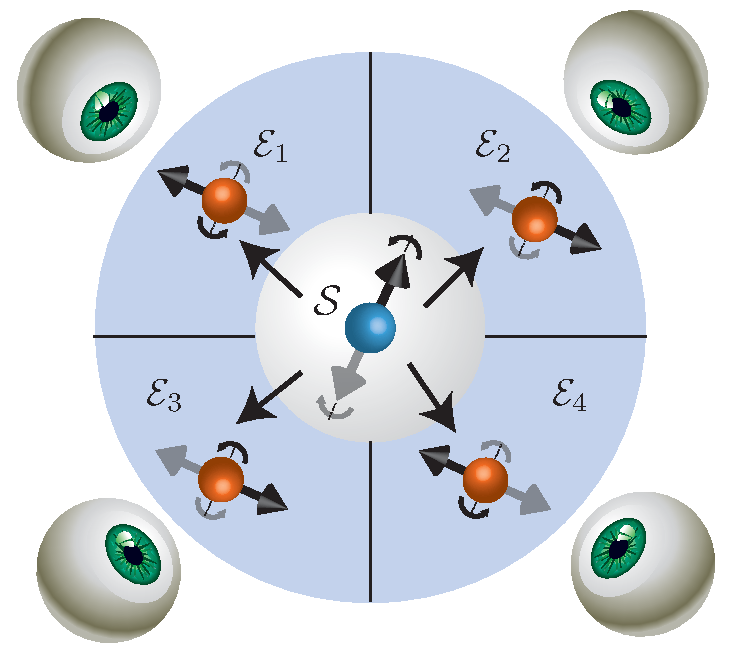
\psfig{file=figure/fig1.pdf, width=0.8\linewidth}}
\caption{The nuclear spin environment as a quantum communication channel. A central electronic spin -- the system $\S$ -- is surrounded by multiple nuclear spins $\E_k$ comprising the environment $\E$. The environment spins are effectively isolated from each other due to their weak spin-spin interaction. The \DIFaddbeginFL \DIFaddFL{interaction between the central spin and an individual nuclear spin is mediated by the hyperfine interaction and depends on the relative position of each spin. The hyperfine interaction strength is therefore different for each nuclear spin. The }\DIFaddendFL environment decoheres the system and, in the process, each of its components is rotated into a new state (black and grey arrows) conditional on the central spin state. Multiple observers (eyes) can access different environment spins and thus independently deduce the state of the system.}
\label{fig:1}
\end{figure}

We will focus on the single electron spin in an NV center~\cite{DOHERTY20131,PSSA:PSSA200671403}, Fig.~\ref{fig:2}a, embedded in a room-temperature diamond environment that carries nuclear $^{13}$C spins (with the natural abundance of 1.1 \%). \DIFaddbegin \DIFadd{The diamond sample is grown via Chamical Vapor Deposition (CVD) and single NV center are introduced into the diamond from residual nitrogen in the CVD plasma. }\DIFaddend Such a platform - a central electron spin coupled to nuclear ancilla spins - has also been studied in previous experiments in different contexts \cite{Taminiau14,Hirose16,Zaiser16}. In the secular approximation~\cite{Childress281}, the Hamiltonian is 
\begin{equation}
\H = 2\pi S_z\sum_k A^k_\parallel I^k_z ,
\label{eq:H0}
\end{equation}
where $S_z = \proj{\up}{\up}$ is a shifted $z$-operator for the electron spin, $I^k_z$ is the spin-1/2 operator for the nuclear spin $k$ and $A^k_\parallel$ the parallel component of the hyperfine interaction (HF) vector $\vec{A}^k$. This is of the pure decoherence form, where environment components interact with the system and do not interact with each other~\cite{Zwolak14,zwolak16,Riedel12-1}. The eigenstates of $S_z$\DIFdelbegin \DIFdel{give }\DIFdelend \DIFaddbegin \DIFadd{, are }\DIFaddend the so-called pointer states of the system~\cite{Zurek81-1}\DIFdelbegin \DIFdel{, the }\DIFdelend \DIFaddbegin \DIFadd{. The }\DIFaddend states that are not perturbed by the environment \DIFdelbegin \DIFdel{but for which superpositions are decohered}\DIFdelend \DIFaddbegin \DIFadd{even though their superpositions decohere}\DIFaddend . For an initial state where the electron spin is in a \DIFdelbegin \DIFdel{``weird'' }\DIFdelend \DIFaddbegin \DIFadd{non-classical }\DIFaddend quantum superposition, $\ket{+}=\ket{\up}+\ket{\down}$, and in a product state with the environment spins (individually in an initialized state $\ket{\phi_k}$), 
\begin{equation}
\ket{\psi(0)} = \ket{+}_\S \otimes \left[ \bigotimes_k \ket{\phi_k} \right],
\label{eq:Psi0}
\end{equation}
the state after evolving for a time $t$ is
\begin{equation}
\ket{\psi(t)} = \ket{\up}_\S \otimes \left[ \bigotimes_k \ket{\phi_{k|\up}} \right] + \ket{\down}_S \otimes \left[ \bigotimes_k \ket{\phi_{k|\down}} \right].
\label{eq:GHZ}
\end{equation}
The superposition in the system has ``branched out'' into the environment, creating correlations with the nuclear spins via conditional rotations into the states $\ket{\phi_{k|\hat{s}}}$ with $\hat{s}=\up,\down$ the pointer states of the system (the $m_s =0$ and $-1$ states of the NV center, respectively, see Fig.~\ref{fig:2}a). 

When $\ket{\phi_k} = \ket{+}$, $A^k_\parallel=A_\parallel$, and $t=1/(2A_\parallel)$, the state in Eq.~\eqref{eq:GHZ} is a GHZ state, where each environment spin holds a perfect record of the pointer state, i.e., the conditional states $\ket{\phi_{k|\up}}$ and $\ket{\phi_{k|\down}}$ are orthogonal \DIFaddbegin \DIFadd{and thus the system's pointer state can be inferred exactly}\DIFaddend . Under more general conditions, the state is GHZ-like and each spin only holds a partial record of the system's state. In either case, \DIFdelbegin \DIFdel{it carries redundant information which }\DIFdelend \DIFaddbegin \DIFadd{the information }\DIFaddend can be quantified by the quantum mutual information between the system $\S$ and a fragment $\F$ of the environment, 
\begin{equation} \label{eq:MI}
\MI = \ES + \EF - \ESF ,
\end{equation}
where $H_\A=-\tr \rho_\A \log_2 \rho_A$ is the von Neumann entropy of subsystem $\A$. This decomposes into classical and quantum components~\cite{Zwolak13-1}, 
\begin{equation} \label{eq:QC}
\MI = \Hol + \QD \DIFdelbegin \DIFdel{,
}\DIFdelend \DIFaddbegin \DIFadd{.
}\DIFaddend \end{equation}
\DIFdelbegin \DIFdel{with
}\begin{displaymath}
\DIFdel{\Hol = \EF - \sum_{s} p_s \CEF(t)
}\end{displaymath}%DIFAUXCMD
\DIFdel{giving }\DIFdelend \DIFaddbegin \DIFadd{The first component is }\DIFaddend the Holevo quantity \DIFdelbegin \DIFdel{-- an upper bound on }\DIFdelend \DIFaddbegin \DIFadd{\mbox{%DIFAUXCMD
\cite{Holevo73,Nielsen11}
}\hspace{0pt}%DIFAUXCMD
}\begin{equation}
\DIFadd{\Hol = \EF - \sum_{s} p_s \CEF(t) ,
}\end{equation}
\DIFadd{which upper bounds }\DIFaddend the classical information \DIFdelbegin \DIFdel{about }\DIFdelend \DIFaddbegin \DIFadd{communicated by a quantum channel, i.e., here, information about the }\DIFaddend observable $\Pi_{\S}$ on \DIFaddbegin \DIFadd{the system }\DIFaddend $\S$ communicated by \DIFaddbegin \DIFadd{an environment fragment }\DIFaddend $\F$\DIFdelbegin \DIFdel{-- and }\DIFdelend \DIFaddbegin \DIFadd{. The second component, }\DIFaddend $\QD$\DIFdelbegin \DIFdel{giving }\DIFdelend \DIFaddbegin \DIFadd{, gives }\DIFaddend the quantum discord~\cite{Zurek00-1,Ollivier02-1,Henderson01-1}. The quantity $\CEF$ is the entropy of $\F$ conditioned on outcome $s$ in $\S$ (with probability $p_s$). 
\DIFaddbegin 

\DIFaddend In principle, one can examine the information about any observable of $\S$, but under decoherence it is information about the pointer states of $\S$, $\PO$ ($S_z$ in our case), that is imprinted on $\F$~\cite{Ollivier04-1,Zwolak13-1}. In what follows, we will determine $\HolpIL$ in a natural setting. 
\DIFdelbegin \DIFdel{Since we are ultimately concerned with the emergence of classical objectivity in natural settings, the quantum information   , }\DIFdelend \DIFaddbegin \DIFadd{We focus on the Holevo information because its complement in the equation for mutual information   -- quantum discord }\DIFaddend $\QDpIL$ \DIFdelbegin \DIFdel{, is difficult to access due to the interactions with many environment spins inaccessible to the measurement, as well as the complexity of the measurement itself.
}\DIFdelend \DIFaddbegin \DIFadd{-- describes correlations between $S$ and $F$ that cannot be shared by observers \mbox{%DIFAUXCMD
\cite{Zurek13}}\hspace{0pt}%DIFAUXCMD
, and, hence, cannot help establish objective reality.
%DIF > Since we are ultimately concerned with the emergence of classical objectivity in natural settings, the quantum information, $\QDpIL$, is difficult to access due to the interactions with many environment spins inaccessible to the measurement, as well as the complexity of the measurement itself. 
}\DIFaddend We thus focus only on $\HolpIL$ and will discuss possibilities for obtaining $\QDpIL$ afterward.

\begin{figure*}
\centerline{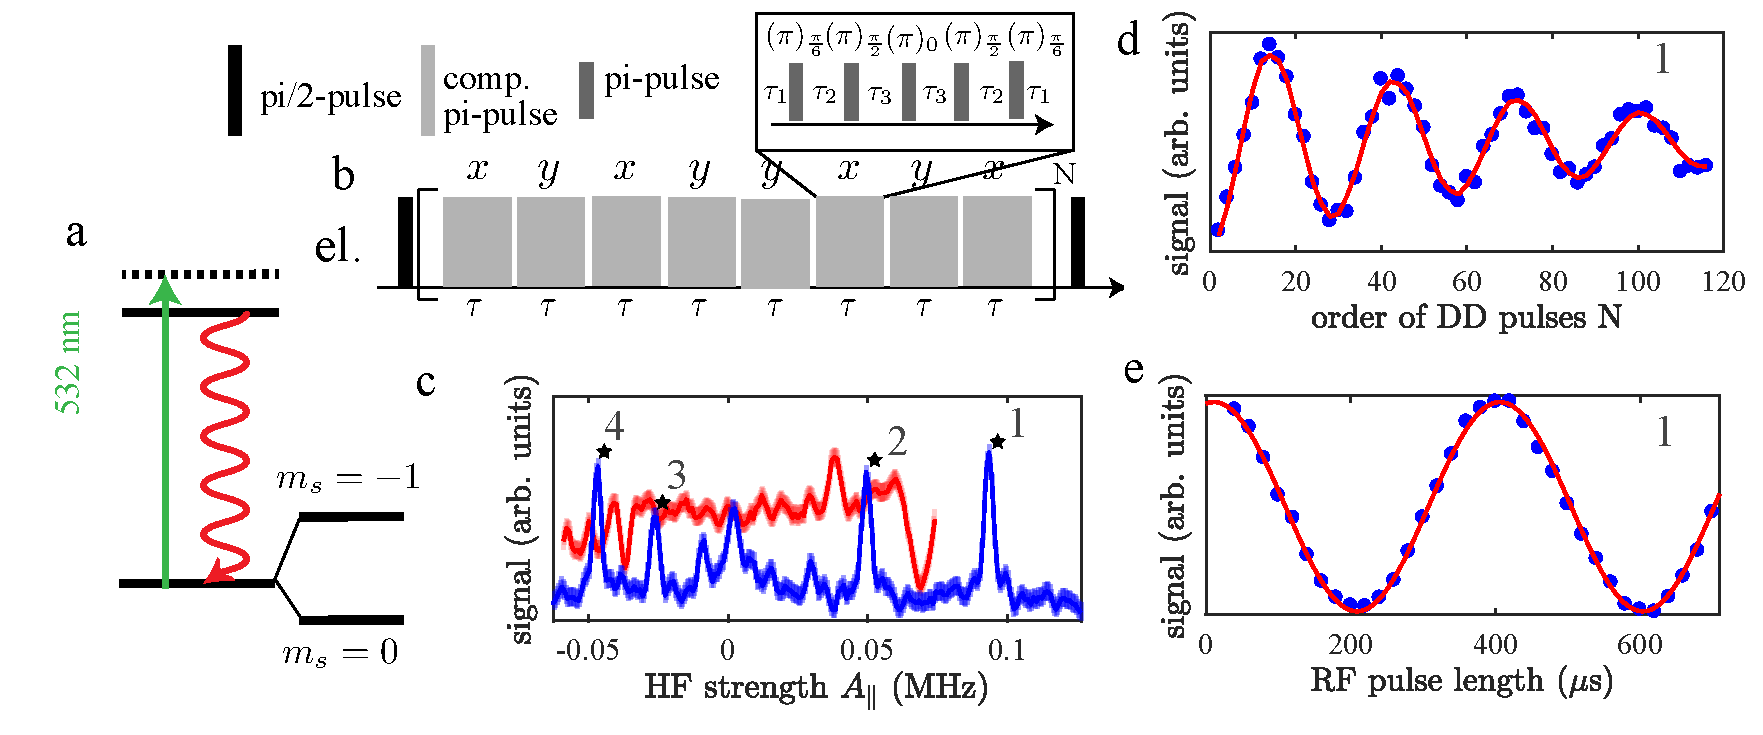
\psfig{file=figure/fig2.pdf, width=1\linewidth}}
\caption{Experimental control of the nuclear-electronic spin system. (a) Energy level diagram of the electronic spin of a NV center. The orbital configuration can be optically excited with green laser light and the passage through the excited state is manifested by red fluorescence. Each orbital state carries a spin triplet ($S=1$) manifold. Spin-dependent non-radiative decay can be used for optical spin detection and efficient spin initialization of the ground state spin sublevel $\ket{m_s = 0}$. In this work we focus on the two-level-system specified by the ground state spin sublevels $\ket{m_s=0} \equiv \ket{\up}$ and $\ket{m_s=-1} \equiv \ket{\down}$. (b) The adaptive XY8$^N$  sequence. The DD sequence is a train of composite $\pi$-pulses with a single pulse duration of $\tau$ and an alternating orthogonal phase (here $x$ and $y$) for robustness. Each composite $\pi$-pulse is a symmetric sequence of five microwave $\pi$-pulses (inset) with different pulse phases to achieve robustness against single pulse imperfections. (c) Measured spectrum (blue) when the interpulse spacing $\tau = 1/(\omega_L+A_{\parallel}/2)$ of an AXY$^{16}$ sequence varies, where $\omega_L$ specifies the bare Larmor frequency of nuclear carbon spins determined by the external, applied magnetic field (here, $\approx 440$ G). For comparison, the result of a standard XY8$^{16}$ spectrum is shown in red. The solid lines are smoothed data and the light blue/red shaded regions represent one standard deviation. \DIFaddbeginFL \DIFaddFL{The four strongest coupled nuclear spins are marked by stars with corresponding numbers and the parallel hyperfine coupling strengths $93.5$ kHz, $49.5$ kHz, $-26.3$ kHz and $-47.1$ kHz are identified. }\DIFaddendFL (d) NV spin mediated Rabi oscillations of a single nuclear spin. The interpulse spacing $\tau$ is tuned to the Larmor period of carbon spin 1 and the order $N$ of the AXY sequence is increased. The red curve is the result of a simulation, when the measured hyperfine values (see section \RN{3} in the SI) are taken into account. (e) Rabi oscillation of nuclear spin 1 driven by a RF field. AXY sequences are used for initialization and readout of the nuclear spin (see section \RN{1} in the SI for more information). The solid curve is a cosine fit corresponding to a sum of squares error (SSE) of $2.4\cdot10^{-4}$. Errors are smaller than the data points in (d,e).}
\label{fig:2}
\end{figure*}

In the case of \DIFaddbegin \DIFadd{the generation of }\DIFaddend a perfect GHZ state (see artificial, experimental creation in section \RN{4} of the SI), the Holevo information is 1 bit for any fragment of the environment: \DIFdelbegin \DIFdel{If there are, e. g.}\DIFdelend \DIFaddbegin \DIFadd{The original system's state is perfectly decohered and each environment spin carries a record of the system's pointer state. Thus}\DIFaddend , several observers which each intercept one spin from the environment, they can all independently determine the \DIFdelbegin \DIFdel{(pointer ) }\DIFdelend \DIFaddbegin \DIFadd{pointer }\DIFaddend state of the system. This is the notion of redundancy, that there are (in this ideal case) $\Es$ copies of the information about the system in the environment of size $\Es$. Departing from ideality, the redundancy, $R_\delta$, will be $\Es/\Fd$ where $\Fd$ is the size of the typical fragment required to \DIFdelbegin \DIFdel{get to }\DIFdelend obtain
\begin{equation} \label{eq:Red}
\avg{\HolpIL} \ge (1-\delta) \HPB .
\end{equation}
That is, the fragment size, on average, to get more than $\HPB$ of the missing information about $\S$. The quantity $\delta$ is the information deficit -- the finite precision one has to pay for lack of ideality. 

%In the case of a perfect GHZ state, the Holevo information is 1 bit for any fragment of the environment: If there are, e.g., several observers which each intercept one spin from the environment, they can all independently determine the (pointer) state of the system. This is the notion of redundancy, that there are (in this ideal case) $\Es$ copies of the information about the system in the environment of size $\Es$. Departing from ideality, the redundancy, $R_\delta$, will be $\Es/\Fd$ where $\Fd$ is the size of the typical fragment required to get to obtain
%\begin{equation} \label{eq:Red}
%\avg{\HolpIL} \ge (1-\delta) \HPB .
%\end{equation}
%That is, the fragment size, on average, to get more than $\HPB$ of the missing information about $\S$. The quantity $\delta$ is the information deficit -- the finite precision one has to pay for lack of ideality. 

It is clear that to observe this process in the laboratory, one either has to perform full quantum state tomography or, to see that there is redundant information, address the individual nuclear spins. State-of-the-art technology uses Dynamical Decoupling (DD) to \DIFdelbegin \DIFdel{address }\DIFdelend \DIFaddbegin \DIFadd{tackle }\DIFaddend issues such as these. However, selectivity in a spectrally dense environment is still a difficult task. Here, we implement a novel DD protocol, theoretically proposed in Refs.~\cite{Cas2015,Cas17}, to both identify the spin environment and to control individual parts of it. Like well-established DD sequences such as CPMG~\cite{MAUDSLEY1986488} or XY8~\cite{gull90}, the protocol employs repetitive central spin flips via a microwave (MW) drive, where the inter pulse spacing determines the frequency of the control window. However, the new protocol, the adaptive XY8 (AXY8) sequence, establishes a robust control of individual nuclear spins mediated by the central electron spin by arbitrarily shaping the DD control-filter. This refocuses undesired noise, allowing for the identification and control of individual nuclear spins. 

More specifically, control of the filter design is supplied by replacing each single spin flip by a train of five pulses, see the inset of Fig.~\ref{fig:2}b. An alternating rotation axis (phase) of the MW pulses permits a robust operation in the presence of pulse errors. In addition, time evolution during the pulse train models an arbitrary filter response, where the evolution times $\tau_1$, $\tau_2$ and $\tau_3$ are numerically calculated with a specific filter function (see section \RN{1} in the SI). In case that the nuclear Zeeman energy is much larger than the hyperfine coupling strength, the process is modeled by the effective Hamiltonian~\cite{Cas2015}
\begin{equation}
H^k = \frac{1}{2}f_{DD}A_\perp \left(S_z -\frac{1}{2}\right) I^k_x,
\label{eq:EM1}
\end{equation}
when the interpulse spacing $\tau$ matches the corresponding Larmor frequency of nuclear spin $k$. $I_x^k$ is the corresponding nuclear spin-$1/2$ operator in $x$-direction and $f_{DD}$ a variable parameter, determining the DD control filter. 

The effective interaction strength $\frac{f_{DD}\A_\perp}{2}$ is mediated by the perpendicular HF coupling $A_\perp$, which is here determined by the magnetic dipole-dipole interaction. Instead of a constant interaction strength, determined by $A_\perp$, a weaker effective strength can be modeled without the necessity of using higher harmonics~\cite{Childress281,Tam14}, which are more vulnerable to pulse error, to achieve individual nuclear spin addressing. \DIFaddbegin \DIFadd{Further experiments (see section }\RN{1} \DIFadd{of the SI) perfomed with different filter coefficients confirm the concept of the AXY sequence and artefacts coming from contributions of higher harmonics can be neglegted due to a large detuning.  }\DIFaddend An AXY spectrum (with $f_{DD}=0.2$) of the nuclear spin environment is shown in Fig.~\ref{fig:2}c (blue curve). Due to electron-nuclear spin entanglement governed by Eq.~\eqref{eq:EM1}, four \DIFdelbegin \DIFdel{nuclear spin }\DIFdelend \DIFaddbegin \DIFadd{stronger coupled nuclear spins }\DIFaddend and additional, more weakly coupled ones can be identified by their different parallel HF interaction strength, when the interpulse spacing $\tau$ varies. The effective coupling strength was here reduced by about a factor of five compared to the \DIFdelbegin \DIFdel{natural }\DIFdelend \DIFaddbegin \DIFadd{dipolar HF interaction }\DIFaddend strength determined by the register geometry. The result of the typical, non-adaptive XY8 sequence (red curve) doesn't show the features. The \DIFdelbegin \DIFdel{natural }\DIFdelend \DIFaddbegin \DIFadd{HF }\DIFaddend interaction strength is too strong, and therefore the resonances too broad to identify individual spins. The rising and falling of quantum correlations between the electronic spin and a nuclear spin is shown in Fig.~\ref{fig:2}d, when the repetition $N$ of the pulse sequence is increased, while the pulse spacing is kept constant and on resonance with the Larmor period of nuclear spin one. In addition, the result in Fig.~\ref{fig:2}e shows a Rabi oscillation of nuclear spin one induced by a resonant radio frequency (RF) field, when a iSwap gate \cite{Cas17} based on the AXY sequence is used for nuclear spin initialization and readout (see more information in section \RN{1} of the SI). 

\begin{figure*}
\centerline{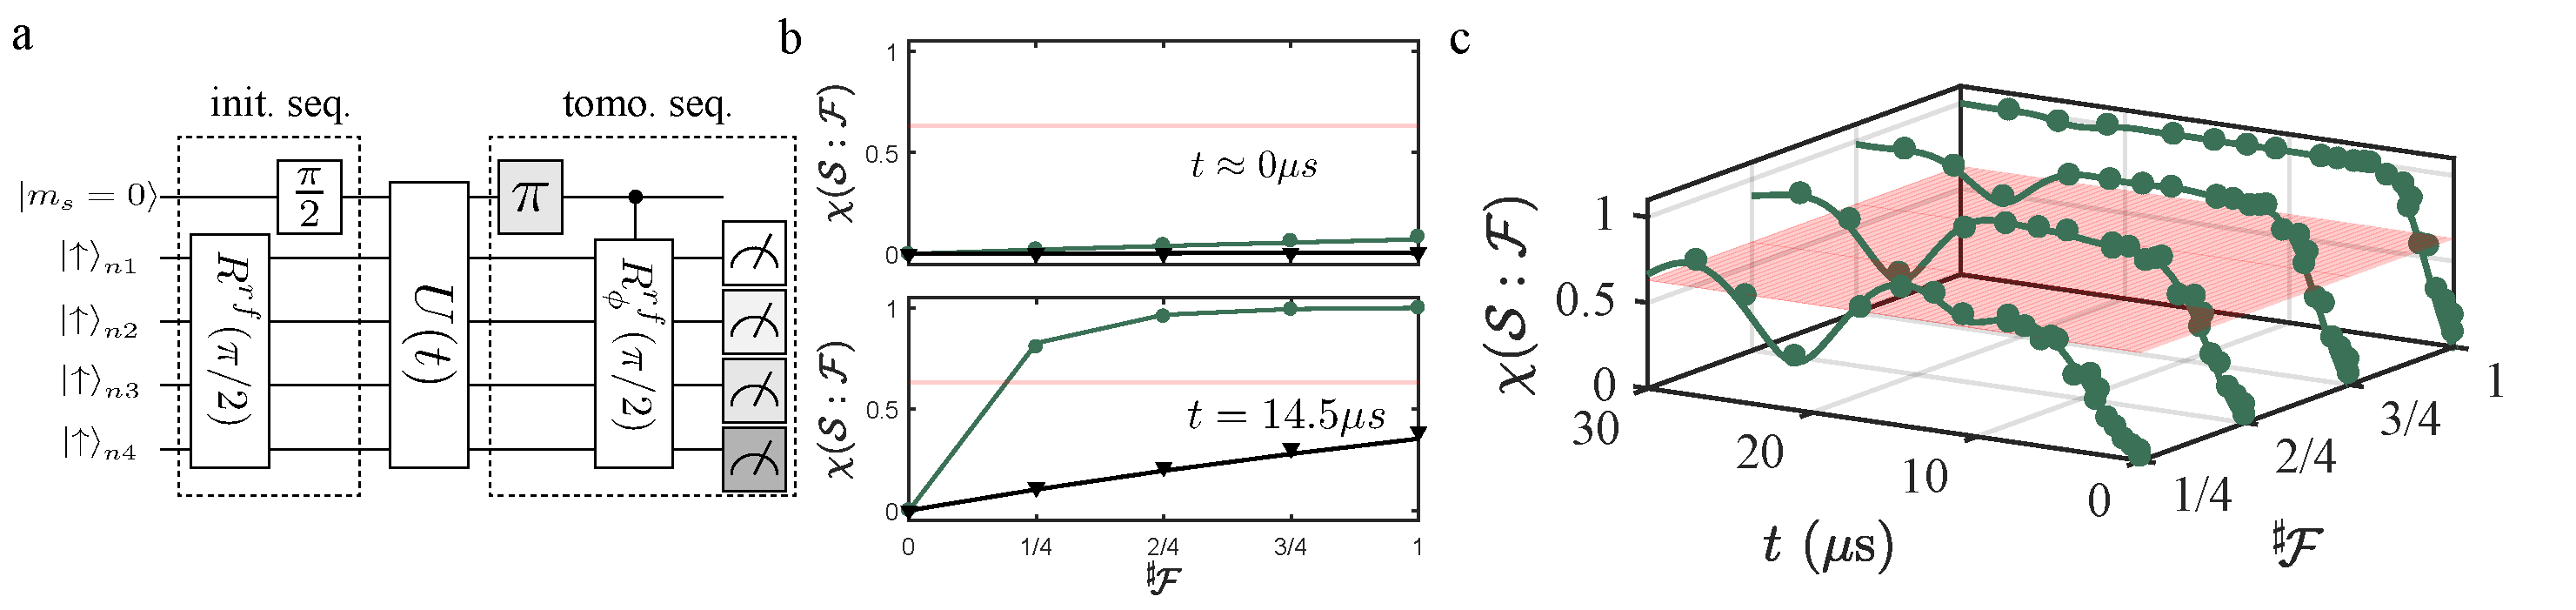
\psfig{file=figure/fig4.pdf, width=1\linewidth}}
\caption{The emergence of redundancy for an NV center being naturally decohered by its environment. (a) The NV spin is first initialized optically and its polarization swapped to each individual nuclear spin by a repetitive process (not shown). Two $\frac{\pi}{2}$-pulses transform the product state into a product state of $\ket{+}$ states. These then evolve under the direct HF interaction between the NV center and nuclear spins ($U(t)$). Single nuclear spin tomography in the electronic subspace $\ket{m_s=-1}$ is performed by a selective $\frac{\pi}{2}$-pulse mediated by a weak, resonant RF pulse ($R^{rf}_{\phi}$). In addition, multiple measurements are performed with different RF pulse phases $\phi$ to determine the phase of the nuclear spin superposition. An optional $\pi$-pulse in front of the last RF pulse can be applied for nuclear spin tomography in the electronic $\ket{m_s=0}$ subspace. The state of a single nuclear spin is in the end swapped to the NV spin and an optical readout follows. (b) Holevo information versus fraction size for two different free evolution times. (c) Holevo information, $\HolpIL$, versus the environment fragment size $\Fs$ and free evolution time $t$. The solid curves in (b) and (c) show the results of simulations with and without imperfect initial polarization. The dynamics in the simulation are governed by the Hamiltonian $H_0$, Eq.~\eqref{eq:H0}. The semi-transparent red lines in (b) and the plane in (c) indicate an information deficit of $1/e$, i.e., $I = (1-1/e) H_\S$. Errors are smaller than the data points.}
\label{fig:4}
\end{figure*}

In previous work, redundancy was created artificially via the construction of a GHZ state, which was achieved for example recently with photonic simulators~\cite{Ciampini18-1,Chen18-1}. In addition, work \DIFdelbegin \DIFdel{on }\DIFdelend \DIFaddbegin \DIFadd{in }\DIFaddend the field of quantum non-demolition (QND)  measurements \cite{Nogues99,Gleyzes07,Lupascu07,Neumann542} were also able to create highly redundant states by consecutive two-body scattering. However, in our everyday world, redundancy appears as a consequence of natural interactions between an $\S$ and $\E$ initially out of equilibrium. To observe this in NV centers, we allow in the following the system to evolve freely in the presence of the natural HF interaction. \DIFaddbegin \DIFadd{Because the effect of the nuclear spin environment on the central electron spin is dominated by the nuclear spins close to the central spin, we concentrate on the four strongest coupled nuclear spins (see Fig.~\ref{fig:2}c). }\DIFaddend The experimental protocol is shown in Fig.~\ref{fig:4}a. We first initialize the system into the out-of-equilibrium product state, Eq.~\eqref{eq:Psi0}, with $\ket{\phi_k}=\ket{+}$. This is followed by the free evolution of $\S\E$ of duration $t$ according to the HF Hamiltonian, Eq.~\eqref{eq:H0}. To determine the classical correlations of fragments, $\F$, of the environment with $\S$, tomography is applied by an electron spin-selective nuclear RF pulse with variable phase $\phi$, which rotates only an individual nuclear spin (see the section \RN{2} and \RN{4} in the SI for more information). Nuclear spin initialization and readout is achieved by a nuclear spin selective iSwap gate mediated by the AXY sequence.

Figure~\ref{fig:4}b shows the Holevo information versus fraction size for two different evolution times and Fig.~\ref{fig:4}c shows the full data set. \DIFdelbegin \DIFdel{The dark green data show the results when error due to an imperfect polarization and tomographyare corrected }\DIFdelend \DIFaddbegin \DIFadd{When errors happen during the nuclear spin polarization as well as tomography, and both sorts of errors are corrected in the analysis }\DIFaddend (see section \RN{2} of the SI)\DIFdelbegin \DIFdel{. When error happening during the initialization are not taken into account}\DIFdelend \DIFaddbegin \DIFadd{, the results are shown in dark green. When only the errors of an imperfect tomography are corrected in the analysis}\DIFaddend , the data is presented in black. Here we focus on the dark green data set. At short times, there is essentially no information in fragments or even the whole environment, as initially the $\S\E$ state is a product state. As time develops, however, information is rapidly transferred into the environment. At a time of 14.5 $\mu s$ even a single nuclear spin captures nearly complete information, to within an information deficit of $1/e$ bits. In other words, all the four most strongly coupled nuclear spins have nearly a complete record of the system's pointer state. This redundancy is \DIFdelbegin \DIFdel{signified by }\DIFdelend \DIFaddbegin \DIFadd{reflected in }\DIFaddend the presence of a plateau in the Holevo information versus fragment size. We note also that the timescale of information rising (on the order of several $\mu$s) is in good agreement with the NV spin coherence time measured by a Ramsey experiment, see section \RN{7} in the SI. With increasing time, though, small fragments will see information flow back into the system. This is due to the fact that for individual spins the conditional states first get rotated away from each other and then back towards each other. For sufficiently large number of spins with random interaction strengths, even this information flow into a single spin will be one way on average. For larger fragment sizes, the information tends more and more to be one way, although there will still be periods of recurrence for long enough waiting times. When the experimental data are not normalized with respect to the initial degree of polarization (black data), redundancy is suppressed due to the lower -- but nonzero except for cases of measure zero~\cite{Zwolak14,zwolak16} -- information capacity of the ``hazy'' environmental fragments~\cite{Zwolak09,Zwolak10-1}. 

We have \DIFdelbegin \DIFdel{focused on }\DIFdelend \DIFaddbegin \DIFadd{exhibited }\DIFaddend the emergence of redundancy under decoherence \DIFdelbegin \DIFdel{. This study , though, gives a path forward to see also the banishment }\DIFdelend \DIFaddbegin \DIFadd{using NV centers. Our study also provides insights to the reason for the selective banishing }\DIFaddend of quantum information\DIFdelbegin \DIFdel{-- the fact that there was initially a superposition that gets transformed into }\DIFdelend \DIFaddbegin \DIFadd{: the initially superposition becomes encoded into the inaccessible }\DIFaddend global quantum correlations. This global coherence leaves a signature in the quantum mutual information ($\QDpIL$, the counterpart to $\HolpIL$ in Eq.~\eqref{eq:QC}) in the form of an ``uptick'' \DIFdelbegin \DIFdel{when the whole (or nearly whole) environment is intercepted}\DIFdelend \DIFaddbegin \DIFadd{a sharp upward turn of the mutual information on the plateau when the fragment size near the total environment size}\DIFaddend ~\cite{Zwolak13-1}. 
%DIF > \todo{The ``uptick''  is a sharp upward turn of the mutual information on the plateau when the fragment size near the total environment size.} 
This can be observed artificially \DIFdelbegin \DIFdel{in, }\DIFdelend e.g., \DIFaddbegin \DIFadd{in }\DIFaddend isolated photonic simulators~\cite{Ciampini18-1,Chen18-1} \DIFaddbegin \DIFadd{and similar settings where couplings between $\S$ and elements of $\E$ are artificially controlled}\DIFaddend . Within natural settings, though, interactions with inaccessible environment components, as well as imperfect readout/initialization of the accessible environment components, make observing the uptick very challenging. Indeed, the inaccessibility of the uptick due to the interactions with many environment components is what makes our everyday world classical~\cite{Zwolak13-1}. Thus, it is no surprise that it is difficult to measure in naturally decohering systems. Further refinement of the DD technique and samples, together with low temperature measurements, may make this uptick accessible. This will motivate future experiments in NV centers embedded in moderately $^{13}$C enriched diamond (see section \RN{8} in the SI) to observe large amounts of redundancy.

\DIFdelbegin \DIFdel{To conclude, these results give }\DIFdelend \DIFaddbegin \DIFadd{Our results provide }\DIFaddend the first laboratory demonstration of quantum Darwinism in action in a natural environment. This \DIFaddbegin \DIFadd{demonstration }\DIFaddend required implementing a novel DD protocol\DIFdelbegin \DIFdel{to observe}\DIFdelend . The process by which nuclear spin decoherence of NV centers gives rise to \DIFaddbegin \DIFadd{incipient }\DIFaddend classical objectivity is \DIFdelbegin \DIFdel{the same as that occurs due to photons }\DIFdelend \DIFaddbegin \DIFadd{analogous to the one that occurs when photons scatter from objects }\DIFaddend in our macroscopic world. In both cases, \DIFdelbegin \DIFdel{the weird }\DIFdelend \DIFaddbegin \DIFadd{flagrantly non-classical (e.g., non-local) }\DIFaddend quantum superpositions are embedded in \DIFdelbegin \DIFdel{a much }\DIFdelend larger environment, initially out of equilibrium. Interactions with the environment select certain preferred \DIFdelbegin \DIFdel{states}\DIFdelend \DIFaddbegin \DIFadd{(pointer) states of the system}\DIFaddend , decohering their superpositions and proliferating accessible information about \DIFdelbegin \DIFdel{them }\DIFdelend \DIFaddbegin \DIFadd{such einselected states }\DIFaddend into the world, \DIFaddbegin \DIFadd{thus }\DIFaddend relegating non-redundant quantum correlations to \DIFdelbegin \DIFdel{the dustbin of inaccessibility}\DIFdelend \DIFaddbegin \DIFadd{inaccessible regions of the Hilbert space}\DIFaddend . Our work shows that already \DIFdelbegin \DIFdel{at }\DIFdelend \DIFaddbegin \DIFadd{on }\DIFaddend the atomic scale \DIFdelbegin \DIFdel{, }\DIFdelend there is evidence of \DIFaddbegin \DIFadd{the process that -- in everyday settings, and for much larger environments -- leads to the emergence of }\DIFaddend classicality. The \DIFdelbegin \DIFdel{presence }\DIFdelend \DIFaddbegin \DIFadd{appearance }\DIFaddend of objective, classical \DIFdelbegin \DIFdel{systems exist therefore in presence of small environments}\DIFdelend \DIFaddbegin \DIFadd{states accessible to indirect measurements is anticipated by processes that take place already in small environments, }\DIFaddend and it simply gets more difficult to avoid \DIFdelbegin \DIFdel{perceiving }\DIFdelend classicality as the environment size grows. This \DIFdelbegin \DIFdel{disfavors other approaches (grav. }\DIFdelend \DIFaddbegin \DIFadd{straightforward and purely quantum account of the origins of the classical in our quantum Universe suggests other approaches to the quantum-to-classical transition (gravitational }\DIFaddend collapse, etc.) \DIFdelbegin \DIFdel{, as those are not intended to describe small 'microscopic' systems}\DIFdelend \DIFaddbegin \DIFadd{are not necessary to describe the emergence of our objective, classical world}\DIFaddend .\\

\section*{\label{sec:Acknowledgement} Acknowledgement}
We thank Jorge Casanova, Zhenyu Wang, Liam P. McGuinness, and C. Jess Riedel for helpful discussions. This work was supported by the DoE LDRD program at Los Alamos National Laboratory, FQX, ERC, VW Stiftung, BW Stiftung, DFG and BMBF\DIFaddbegin \DIFadd{.  WHZ acknowledges partial support by the Foundational Questions Institute grant FQXi-1821, and Franklin Fetzer Fund, a donor advised fund of the Silicon Valley Community Foundation}\DIFaddend . 

\bibliographystyle{apsrev}
\bibliography{reference}

\end{document}

